\documentclass[11pt,a4paper]{article}
\usepackage[utf8]{inputenc}
\usepackage[T1]{fontenc}
\usepackage{graphicx}
\usepackage{amsmath}
\usepackage{hyperref}

\title{Generating provable primes}
\author{Sigurd Meldgaard \and Kasper Damgaard}
\date{17. Dec.}
\begin{document}
\maketitle
\section{Introduction}
Primes are usually generated by testing random numbers for primality
using a randomized prime test (the most popular being the Miller-Rabin
test).  But these tests do not guarantee that the number is prime,
only make it arbitrarily likely.

If we know the factorization of $p-1$ where $p$ is prime, it is
possible to generate a certificate showing the primality of $p$. This
cannot be used to show that a randomly chosen number is prime, but we
can instead generate the prime ``bottom up'' in a recursive way.

By choosing the sizes of the factors of $p-1$ carefully the generated
primes can have an almost uniform distribution. This is of course
important if the primes are used for cryptographic purposes.

This is asymptotically almost as fast as using a Miller-Rabin test for
generating primes of size $n$.

We describe some details of this way of constructing primes, give an
implementation of the algorithm, measure it, and compare it to
generating primes using the Miller-Rabin prima
\section{Theoretical background}
\subsection{Lucas' primality criterion}
Lucas' primality criterion is described in \url{http://www.mathpages.com/HOME/kmath473.htm}

Eulers theorem:
\[
\forall n\in N, k, gcd(k,n)=1: k^{\phi(n)} \equiv 1 \mod n
\]

Given a base $b$ and a prime candidate $n$. Where $b$ fulfills Fermat's equation for primes:
$b^{(n-1)}  \equiv  1    \mod n$

Denote the smallest exponent where the sequence:
\[1, b^2, b^3 ... \mod n\]
reaches $1$, the period of $b$ mod $n$ or $ord_p(b)$. 

We know that 
\[b^{\phi(n)} \equiv 1 \mod n\]
 so 
\[ord_p(b)|\phi(n).\] 
And also that \mbox{$ord_p(b)|(n-1)$} (from the requirement of $b$) or
equivalently $n-1 = x\cdot ord_p(b)$ for some positive integer $x$.

If we can prove $x=1$ then $ord_p(b)=n-1=\phi(n)$ because: $\phi(n) \leq
n-1$, and $n$ must be prime.

Assume we know the factorization of $n-1 = q_1^{\beta_1}q_2^{\beta_2}\ldots q_r^{\beta_r}$.

Then we can check that:
\[b^{(n-1)/q_i}\not\equiv 1 \mod n, i\in{1..r}\] If we raise $b$
to a power not a multiple of $ord_p(b)$ it will be different from $1$,
so $(n-1)/q_i\not|ord_p(b)$ for any $i$, And if that is true all
factors of $n-1$ are not factors of $x$, and therefore $x=1$.
%. Because only primes have
%$\phi(n) = n-1$ 
\subsection{Generating primes bottom up}
For generating large primes we can recursively generate smaller
primes, multiply them and see if the product plus one is a prime by
testing for Lucas' criterion.

For the base case (primes smaller than a certain threshold) we use
trial division of a random number to construct the prime.

Really we only need to know the factorization of $F$, and let:

\[n = 2RF+1\] 

Where $R$ is generated randomly, $F$ is odd and $F>R$, because if $F$
is odd and the test succeeds for some base $b$ the smallest possible
prime factor of $n$ is $2F+1$, and because $F>R$ $n=(2RF+1)<(2F+1)^2$,
$n$ must be prime.

As explained in \cite{DBLP:journals/joc/Maurer95} almost any base will work
for showing the primality of $p$, the exact proportion of good bases
is:

\[\phi(F)/F \geq 1-\sum^r_{j=1}1/q_j\]

A proof is also given in \cite{DBLP:journals/joc/Maurer95} that explains that
it is possible to further enhance the speed of the algorithm. This is done
by defining an equation: $2R = xF + y$, where $0\le y < F$. Then, if we can 
determine that $y^2 - 4x$ is not 0 or a perfect square, we know that n 
is prime if $F$ is just greater or equal to $\sqrt[3]{n}$. However, this
comes with the cost of a slightly distorted uniformity.

To ensure that the primes are generated reasonably uniformly the size
of the smaller primes generated in the recursive calls must be chosen
properly.

In \cite{DBLP:journals/joc/Maurer95} a method is given for choosing the sizes
from the distribution of the relative size of the largest factor of a
random integer $F$. And it is argued that the conditional distribution
given that $2F+1$ is prime is almost the same.

Also it is noted that if $F$ has only one prime factor, we still
choose from among 10 \% of all primes.

The asymptotic estimated running time of finding a $k$-bit prime with the
asymptotically best multi-precision algorithms is:
\[O(k^3\cdot\log\log(k)).\]
For straightforward integer arithmetic the estimated running time is:
\[O(\frac{k^{4}}{\log(k)})\]
\section{The algorithm}
We here present a slightly modified version of the implementation
given in \cite{Menezes:1997:HAC} as algorithm 4.44.\\

\noindent
$\text{PROVABLE PRIME}(k)$\\
INPUT: a positive integer $k$.\\
OUTPUT: a $k$-bit prime number $n$.
\begin{enumerate}
\item (If $k$ is small, then test random integers by trial division. A table of small primes may 
be precomputed for this purpose.) 
If $k \leq 20$ then repeatedly do the following: 
\begin{enumerate}
\item Select a random $k$-bit odd integer n. 
\item Use trial division by all primes less than $\sqrt{n}$ to determine whether $n$ is prime. 
\item If $n$ is prime then return(n).
\end{enumerate}
\item Set $c\leftarrow 0.1$ and $m\leftarrow 20$. 
\item (Trial division bound) Set $B\leftarrow c \cdot k^2$. 
\item (Generate r, the size of q relative to n) If k > 2m then repeatedly 
do the following: select a random number s in the interval [0, 1], set $r\leftarrow 2^{s-1}$ , until 
$(k - rk) > m$. Otherwise (i.e. $k \leq 2m$), set $r\leftarrow 0.5$. 
\item Compute $q\leftarrow \text{PROVABLE PRIME}(\lfloor r \cdot k \rfloor + 1)$. 
\item Set $I \leftarrow \lfloor 2^{k-1} /(2q) \rfloor$. 
\item $success\leftarrow False$. 
\item While (not $success$) do the following:
  \begin{enumerate}
\item (select a candidate integer $n$) Select a random integer $R$ in the interval 
$[I + 1, 2I]$ and set $n\leftarrow 2Rq + 1$. 
\item Use trial division to determine whether $n$ is divisible by any prime number $< B$.

If it is not, do a Miller-Rabin primality test of $n$ with base 2.

If that does not show that $n$ is composite, do the following: 

Select a random integer a in the interval $[2, n - 2]$. 

Compute $b\leftarrow a^{n-1} \mod n$. 

If $b = 1$ do the following: 

\ \ \ Compute $b\leftarrow a^{2R} \mod n$ and $d\leftarrow  gcd(b - 1, n)$.

\ \ \ If $d = 1$ then $success\leftarrow True$.
\end{enumerate} 
\item Return(n). 
\end{enumerate}

\section{Implementation}

We used several optimization tricks noted in \cite{Menezes:1997:HAC}, especially the
execution time was improved much by doing a single Miller-Rabin test
with base 2 of $2FR+1$ before actually testing for Lucas' primality
criterion, this quickly weeds out most of the composites.

For random input we use Pythons built-in Mersenne Twister
implementation, which has fine statistical properties, but is
unsuitable for cryptographic use, this must be changed before the
implementation can be used for such purposes.

We implemented the algorithm in Python (mauer.py), using the built-in
multi-precision integers.  The speed loss due to interpretation is
negligible in this case, as most of the time is spent doing modular
exponentiations. On the other hand a faster MP-library (for example
gmp is possibly a little faster for large bitsizes) will give us
savings.

We also implemented the Miller-Rabin primality test (millerrabin.py),
for comparison.

The program is run as: \verb|python mauer.py 1024| for $k=1024$.

\section{Results}
\begin{figure}[h]
  \centering
  %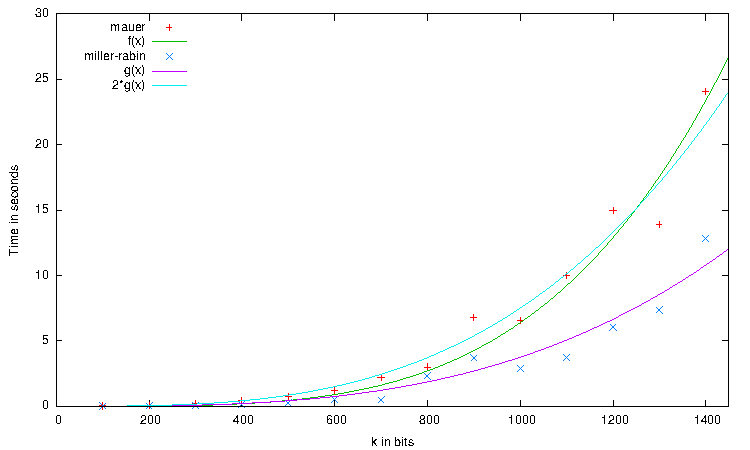
\includegraphics{plot.pdf}
  \caption{Timings of the two prime construction methods}
  \label{fig:timings}
\end{figure}

We have timed 10 runs of each algorithm with different bitlengths (in
the interval 100 to 1400 bits) on a 2.4 GHz Intel core 2 Duo running
Mac OS X, and are giving the average running times in seconds,
measured in CPU-time in user-mode as given by the unix tool
\verb|time|. 

There are big deviations from the average, this is due to the
algorithm depending a lot on ``being lucky'' when choosing the random
parameters.

In the graph we have plotted our average timing plots, and fitted a
$\frac{k^4}{log(k)}$ curve to the Mauer measurings, and a
$k^3\cdot\log(k)$ to the Miller-Rabin.  It is seen from the graph that the Mauer
primality construction in our implementation takes ca. twice as long
as constructing a pseudo-prime with the Miller-Rabin test for primes
around 1024 bits.

For practical purposes one would want to do the Miller-Rabin test for
several bases to make the probability of accepting a composite number
negligibly small.
\section{Conclusion}
Generating provable primes for public key parameters is certainly
practically possible. But Miller-Rabin test is easier to implement and
can construct pseudoprimes with very high certainty in ca. the same
time. And these numbers will be distributed truly uniformly among all
primes.


\bibliography{rapport}{}
\bibliographystyle{authordate1}


\end{document}
